
\section{Краткая характеристика программы} \sectionmark{Краткая характеристика программы}
''VP\_auto'' представляет собой консольную программу. Эта программа предназначена для создания перечней элементов на электрические схемы, спецификаций на печатные платы и ведомость покупных на изделие. Программа не имеет графического интерфейса потому, что её автор не видит целесообразности в его применении в данном случае. При правильно организованном проекте генерация всех выше перечисленных документов производится в одно касание без утомительного кликанья по меню, спискам, окошкам.

Предположительно, что изделие -- это одно законченное электронное устройство (а не сложный комплекс с комплектами ЗИП и др...). Программа скорее предназначена для проекта, содержащего несколько печатных плат и схему верхнего уровня, включающую в себя эти печатные платы. Каждой печатной плате соответствует принципиальная схема. 

Все схемы должны быть выполнены в одном стиле (одинаковые элементы на схемах должны быть названы одинаково с точностью до буквы и пробела). Для контроля за правильностью названий элементов в программе применены несколько механизмов: контроль степени схожести элементной базы внутри проекта и контроль степени схожести с эталонными списками. Контроль степени схожести реализован на основе применения регулярных выражений.

Из принципиальных схем (формат ''P--CAD~2006~SP2 Sсhematic'' и/или ''Altium Designer'') создаются отчёты (bill of material) с информацией о составе и количестве элементов. Эти отчёты обрабатываются программой и в результате создаются:
\begin{itemize}
  \item  заполненные перечни элементов на схемы (формат ''P--CAD~2006~SP2 \\Sсhematic'');
  \item  спецификации на сборки (вернее, графа ''прочие изделия'') (формат \\''P--CAD~2006~SP2 Sсhematic'');
  \item  бирки с названием и количеством элементов для мелкосерийного производства (формат \\''P--CAD~2006~SP2 Sсhematic'');  
  \item  ведомость покупных изделий на всё устройство (формат ''P--CAD~2006~SP2 \\Sсhematic'');
  \item  ведомость покупных изделий в виде текстового файла, пригодного для импорта в электронную таблицу ''MS Excel'' (текстовый файл с разделителями символами табуляции);
  \item  текстовый файл отчёта работы программы, в котором расписано по шагам какие манипуляции были выполнены над входной информацией и на какие записи обратить внимание.
\end{itemize}

Таким образом, минимизируется число несоответствий в этих документах. Наименование и количество элементов в перечне элементов в точности соответствует спецификации и ведомости покупных.

Отметим, что программа делает только 98\% работы за Вас. Остальные 2\% Вы должны проделать сами. А именно: внимательно просмотреть полученные документы, подправить там где надо подправить, не забыть про позиции не обозначенные на принципиальной схеме (держатель вставки плавкой, колпачок на соединитель, радиатор, крепление радиатора и др..).

Для нормальной работы программы необходимы следующие файлы:
\begin{itemize}
  \item библиотечные и исполняемые файлы, содержащиеся в папках \verb|"VP_auto/bin"| и \verb|"VP_auto/plugins"|;
  \item командный файл \verb|"my_path/*.bat"|;
  \item файлы отчётов \verb|"my_path/src/*.bom"| с номенклатурой и количеством покупных изделий (генерируются из ''P--CAD~2006~SP2'' и/или ''Altium Designer'');  
  \item файл с соответствиями имён файлов отчётов и децимальных номеров \\\verb|"my_path/src/*.do"|;
  \item файлы -- заготовки для перечней элементов (\verb|"VP_auto/canvas/per_canvas.sch"|, \verb|"VP_auto/canvas/per_canvas_i1.sch"|), спецификаций (\verb|"VP_auto/canvas/sp_canvas.sch"|), ведомости покупных (\verb|"VP_auto/canvas/vp_canvas.sch"|) в ASCII -- формате среды \\''P--CAD~2006~SP2'' (уже содержатся в каталоге с программой);
  \item шрифт \verb|"GOST_B.TTF"|, установленный в систему (для удобства, помещён в каталог \verb|"./titles"| вместе с шаблонами основных надписей для файлов--заготовок \verb|"*_canvas.sch"|);
  \item ресурсные файлы, доступные для редактирования пользователем (с названием фирм, эталонным списком элементов, списком с единственным/множественным названием элементов) \verb|"VP_auto/res/firms.txt"|, \verb|"VP_auto/res/true_elements.txt"|,
  \verb|"VP_auto/res/names.txt"|.
\end{itemize}





%%%%%%%%%%%%%%%%%%%%%%%%%%%%%%%%%%%%%%%%%%%%%%%%%%%%%%%%%%%%%%%%%%%%%%%%%%%%%%%%%%%

\section{Файлы отчётов} \label{sec:reports} \sectionmark{Файлы отчётов}
\subsection{Файлы отчётов среды ''P--CAD~2006~SP2''}
  Файл отчёта (\verb|"*.bom"|) представляет собой текстовый файл, примерный вид которого показан на рисунке~\ref{p:pic_pcad_low_bom_file}.

\begin{figure}[H]\center
  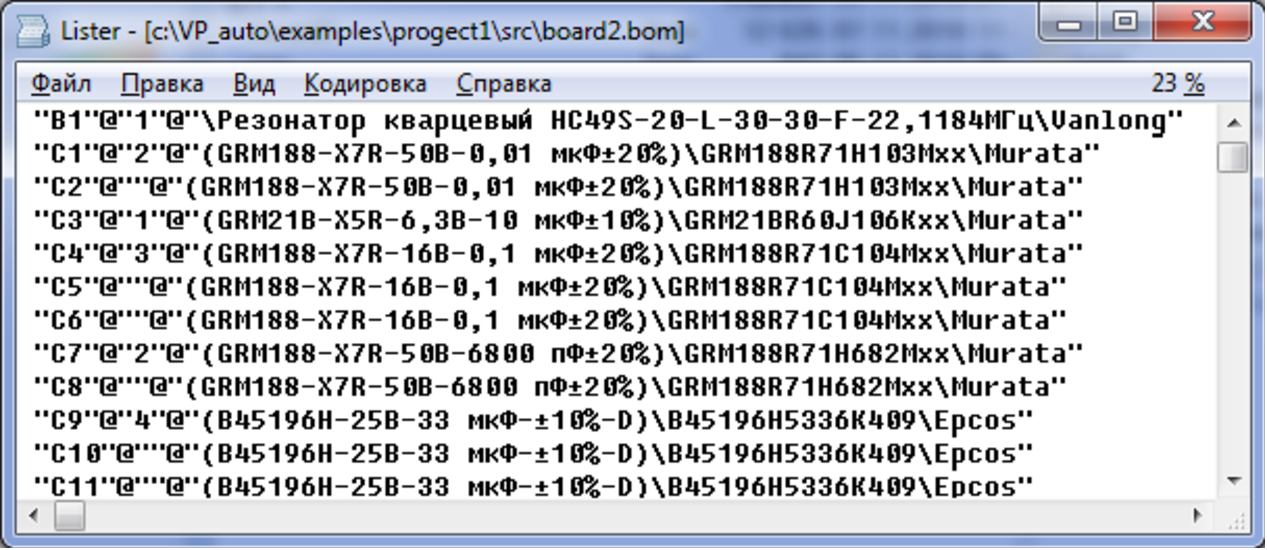
\includegraphics[width=0.8\textwidth]{VP_auto/pictures/pcad/pic_pcad_low_bom_file}
  \caption{Содержимое ''*.bom''--файла, созданного из ''P-CAD 2006 SP2 Shematic''} \label{p:pic_pcad_low_bom_file}
\end{figure}

Для правильного создания такого файла в среде проектирования ''P-CAD 2006 SP2 Shematic'' (рисунок~\ref{p:pic_about_shematic}) нужно выполнить ниже рекомендуемые действия.

\begin{figure}[H]\center
  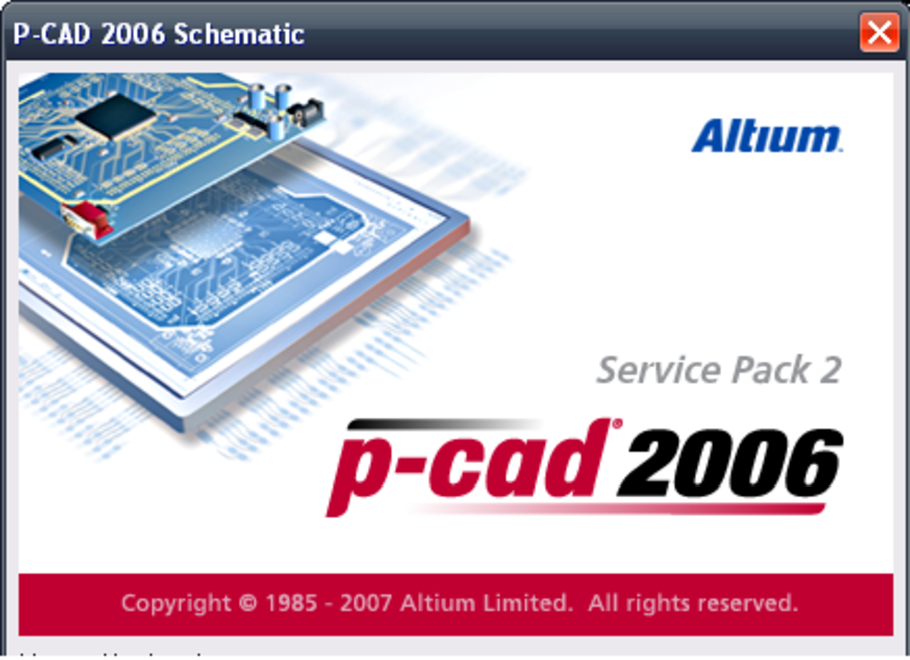
\includegraphics[width=0.5\textwidth]{VP_auto/pictures/pic_about_shematic}
  \caption{Окно ''About'' среды ''P-CAD 2006 SP2 Shematic''} \label{p:pic_about_shematic}
\end{figure}

\newpage
\subsubsection{}Проставить в свойствах каждого элемента в поле \verb|"Value"| текст, который будет фигурировать в ведомости покупных в формате: \\
\fbox{расшифровка\textbackslash код продукта\textbackslash фирма--производитель} \\ \hspace*{20mm} (пример: \fbox{(GRM188-X7R-16В-0,1 мкФ+-20\%)\textbackslash GRM188R71C104Mxx\textbackslash Murata})\\
или \\
\fbox{\textbackslash код продукта\textbackslash фирма--производитель} \\ \hspace*{20mm} (пример: \fbox{\textbackslash 74LVC04 AD\textbackslash Phillips})\\
или \\
\fbox{\textbackslash код продукта\textbackslash технические условия} \\ \hspace*{20mm} (пример: \fbox{\textbackslash Приёмник навигационный\textbackslash АБВГД.123456.074}).

Знак \verb|"\"| является разделителем между полями. Знак \verb|"@"| тоже
зарезервирован. Остальными знаками можно пользоваться. Примерный вид свойств элемента показан на рисунке~\ref{p:pic_pcad_component_properties}). Поле ''расшифровка'' было вынесено на передний план не случайно. При открытии свойств элемента в глаза бросается расшифрованный номинал элемента (сильно облегчает жизнь в случае резисторов и конденсаторов).

\begin{figure}[H]\center
  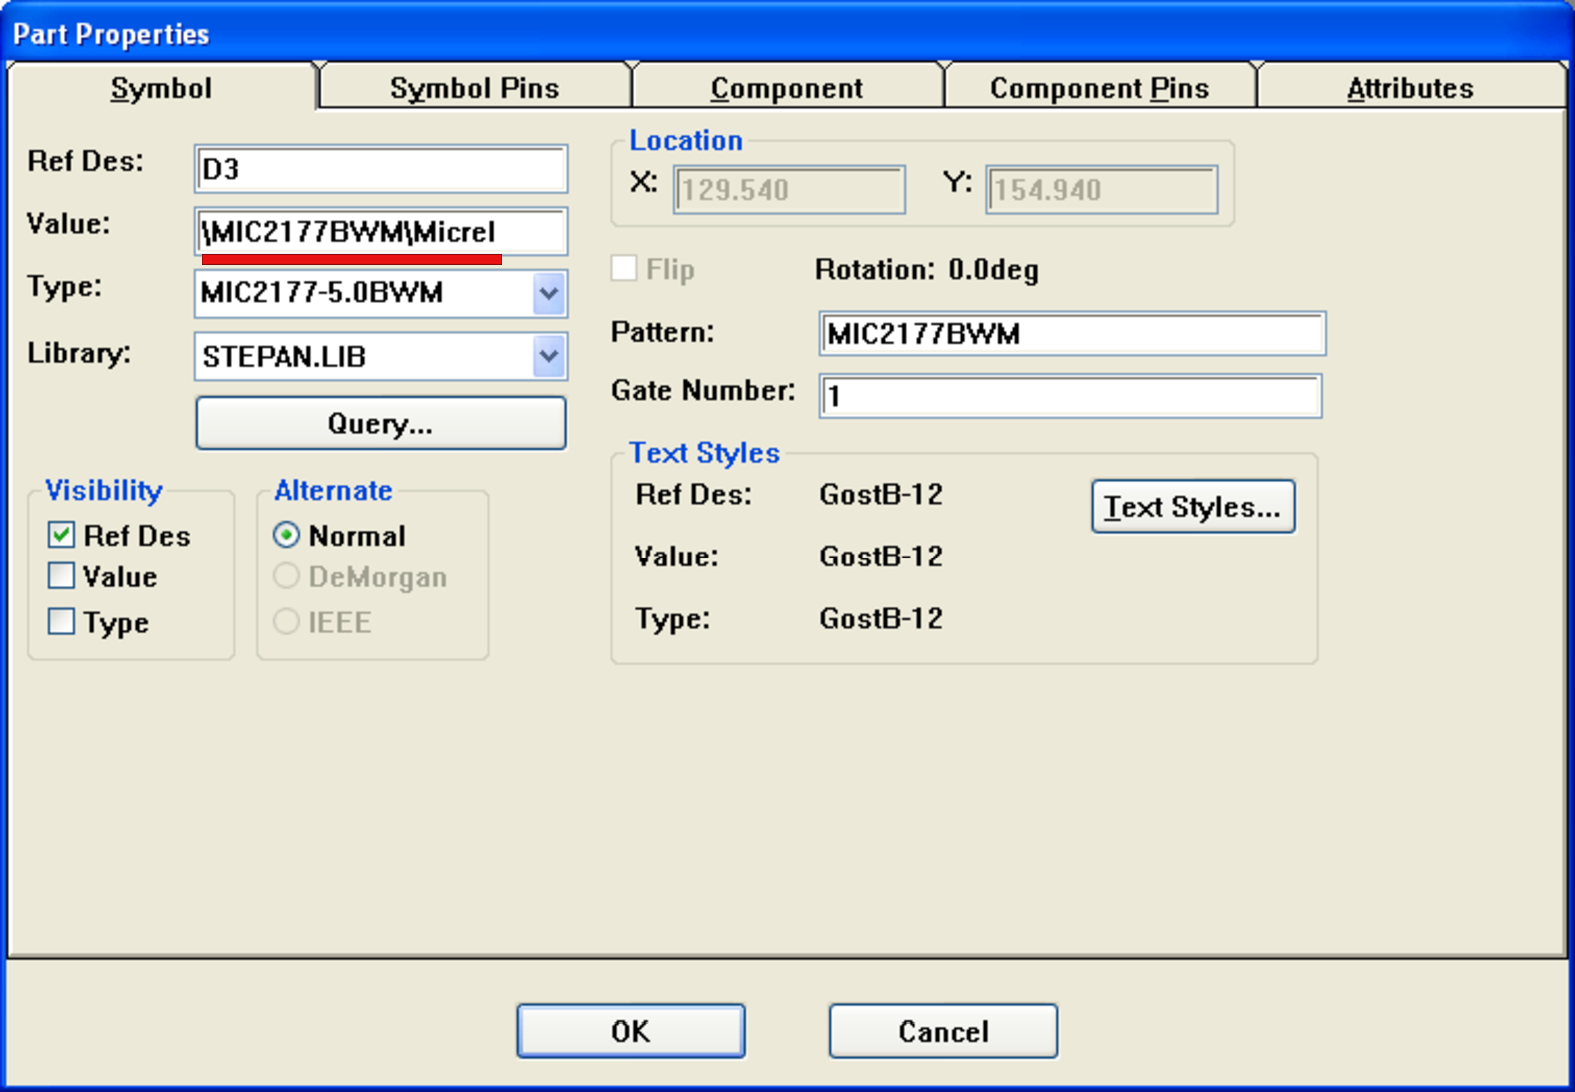
\includegraphics[width=0.8\textwidth]{VP_auto/pictures/pcad/pic_pcad_component_properties}
  \caption{Окно свойств элемента среды ''P-CAD 2006 SP2 Shematic''} \label{p:pic_pcad_component_properties}
\end{figure}

Отметим, что хоть на первый взгляд эта операция может показаться излишне трудоёмкой, но как показала практика -- она жизненно необходима для улучшения качества проекта в целом. Человек, анализирующий схему может мгновенно заглянуть в свойства элемента и узнать его номинал а также типоразмер корпуса, допуски на номинал, температурный разброс и другое... Нет необходимости всё время искать эту информацию в отдельном файле перечня, который действителен только до первой перенумерации. В данном случае перенумерация не страшна. Номинал элемента, который был получен путём расчётов, не переползёт на соседний элемент.

\subsubsection{}Настроить параметры файла отчёта. Заходим в \verb|"File->Reports..."|
и устанавливаем настройки согласно рисунку~\ref{p:pic_pcad_file_report}.

\begin{figure}[H]\center
  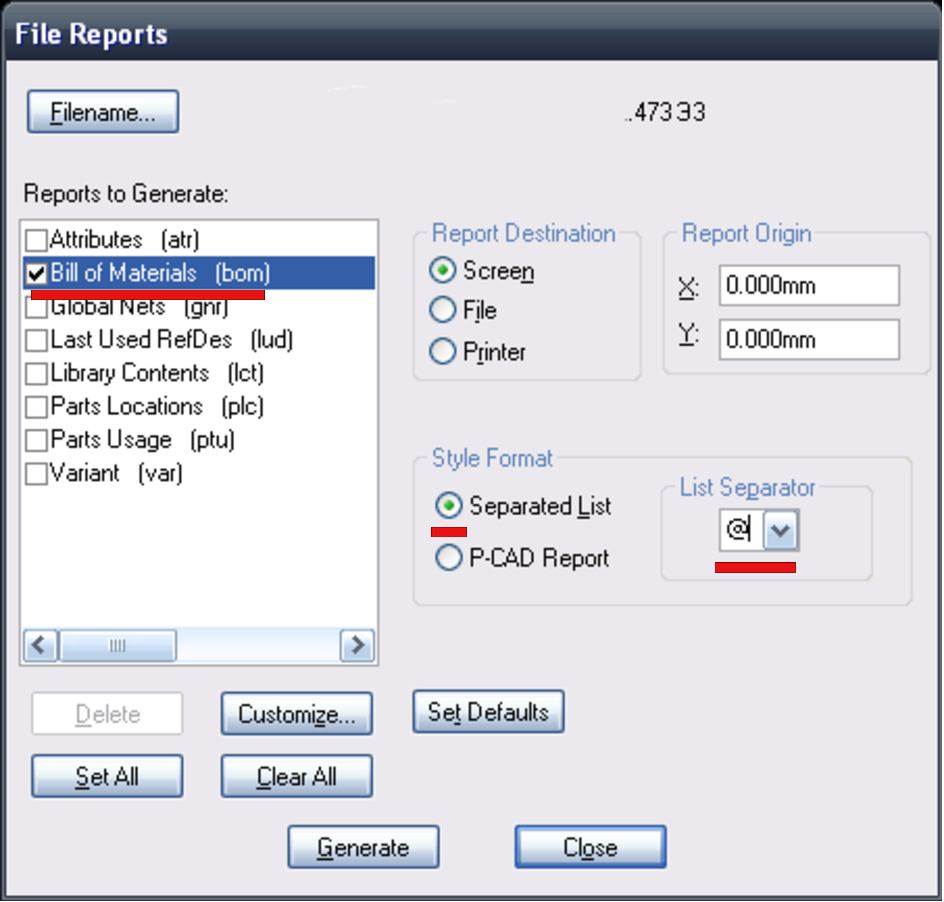
\includegraphics[width=0.8\textwidth]{VP_auto/pictures/pcad/pic_pcad_file_report}
  \caption{Окно выбора типа файла отчёта среды ''P-CAD 2006 SP2 Shematic''} \label{p:pic_pcad_file_report}
\end{figure}

\newpage
Заходим в \verb|"Customize..."| и устанавливаем настройки согласно рисунку~\ref{p:pic_pcad_customize_report_format}, рисунку~\ref{p:pic_pcad_customize_report_selection} и рисунку~\ref{p:pic_pcad_customize_report_sort}

\begin{figure}[H]\center
  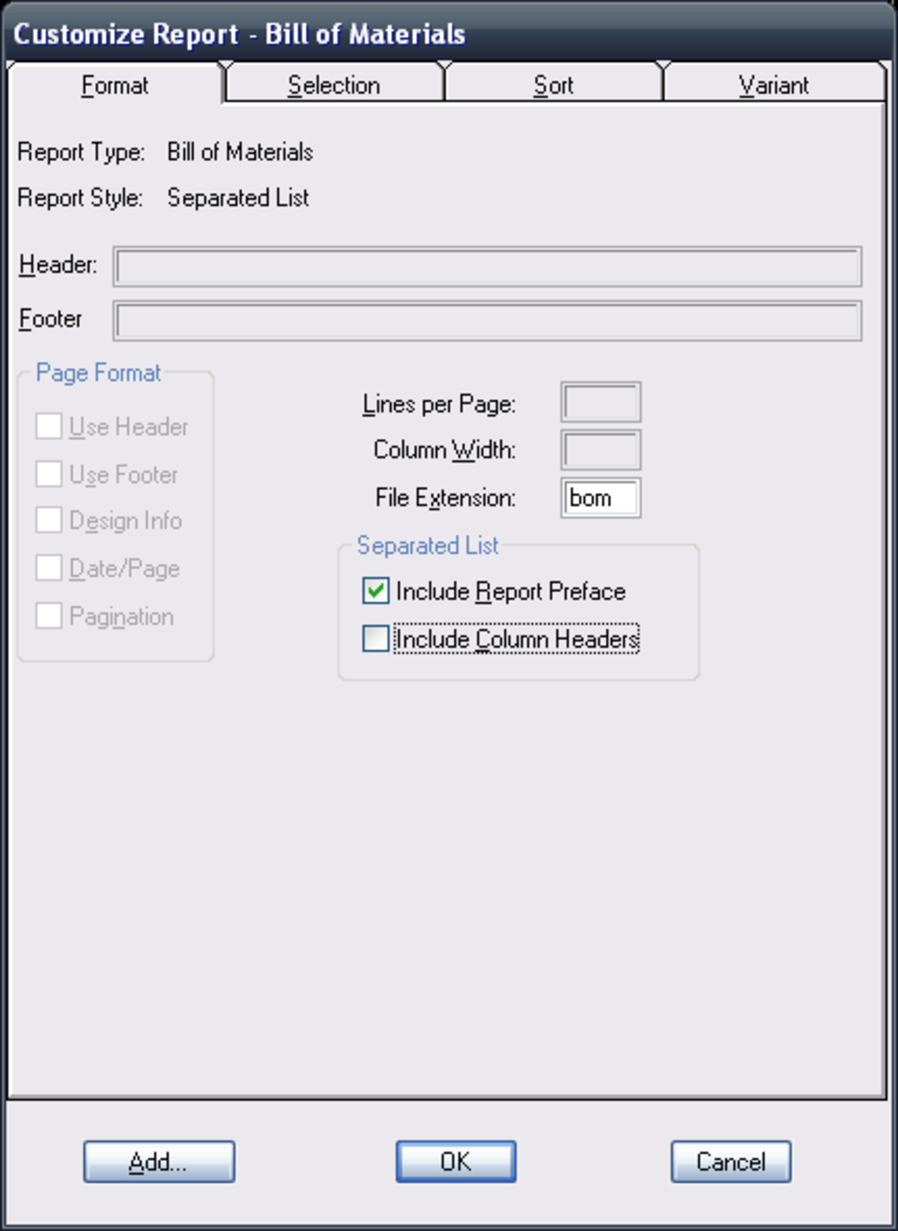
\includegraphics[width=0.8\textwidth]{VP_auto/pictures/pcad/pic_pcad_customize_report_format}
  \caption{Вкладка ''Format'' окна настроек файла отчёта} \label{p:pic_pcad_customize_report_format}
\end{figure}

\newpage
\begin{figure}[H]\center
  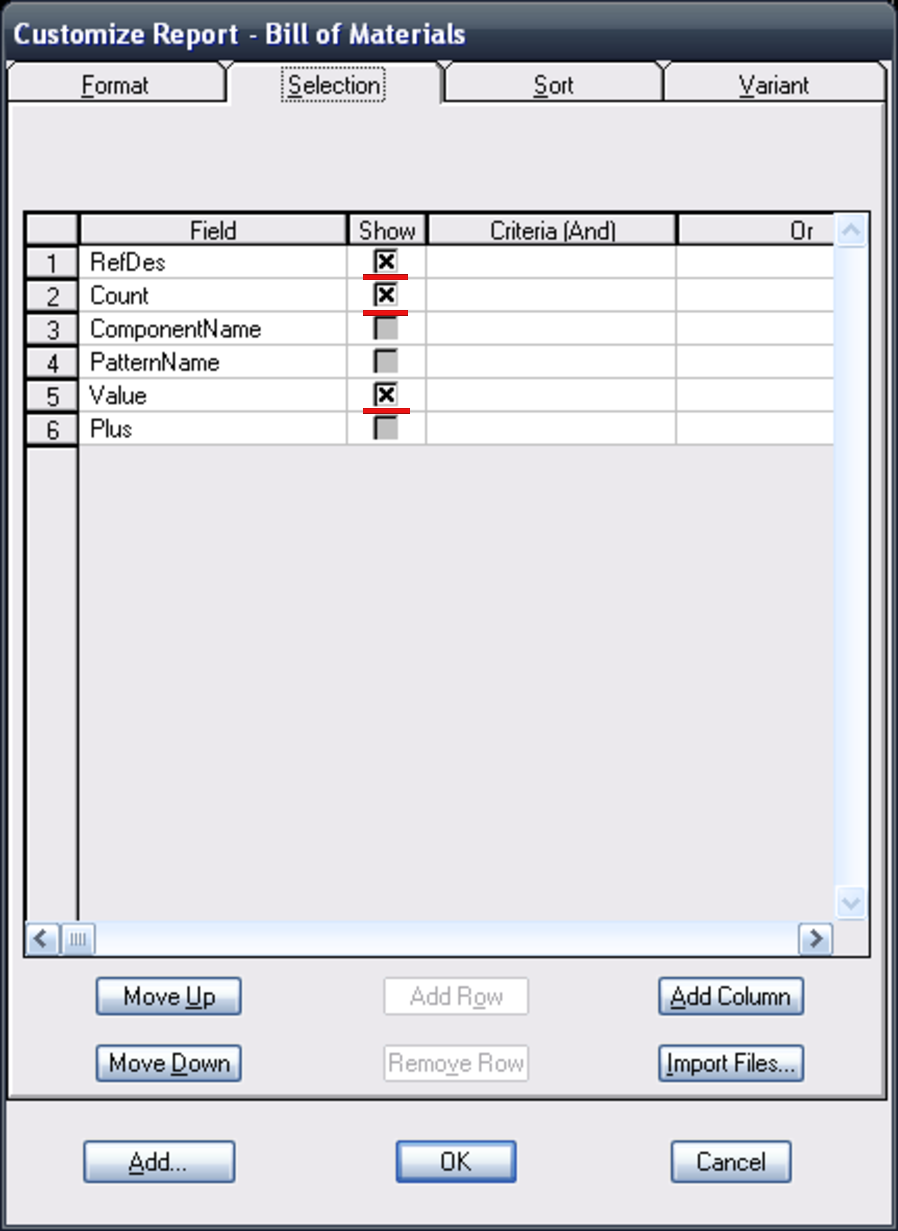
\includegraphics[width=0.8\textwidth]{VP_auto/pictures/pcad/pic_pcad_customize_report_selection}
  \caption{Вкладка ''Selection'' окна настроек файла отчёта} \label{p:pic_pcad_customize_report_selection}
\end{figure}

\newpage
\begin{figure}[H]\center
  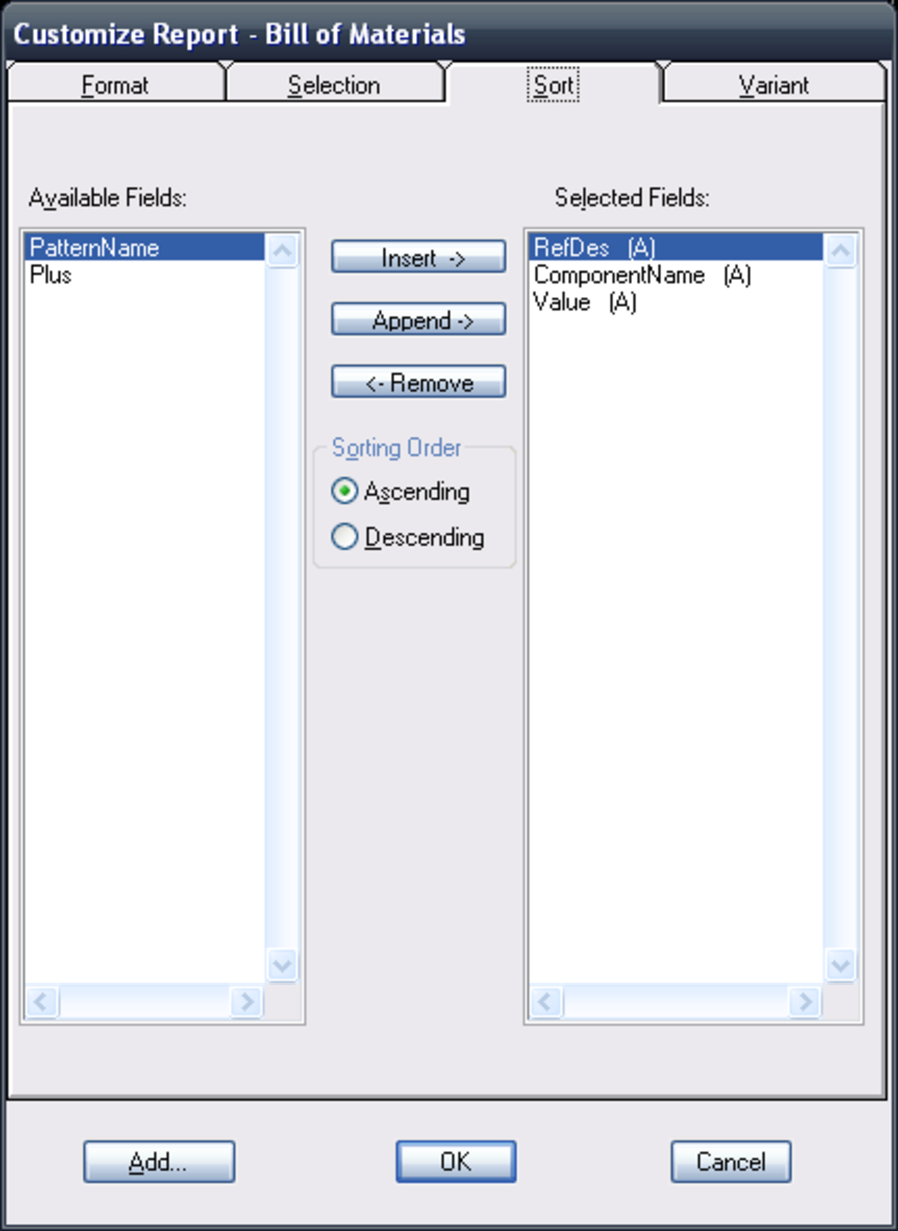
\includegraphics[width=0.75\textwidth]{VP_auto/pictures/pcad/pic_pcad_customize_report_sort}
  \caption{Вкладка ''Sort'' окна настроек файла отчёта} \label{p:pic_pcad_customize_report_sort}
\end{figure}

Создаём файл отчёта и сохраняем его в папке \verb|"my_path/src/"|.

\subsubsection{}Проделываем аналогичные операции с остальными файлами.

Отметим, что в принципе можно было сделать так, чтобы программа извлекала информацию о элементах схемы из самого схемного \verb|"*.sch"| -- файла (не так уж сложно всё отсортировать там), но это влекло бы к дополнительным ошибкам в номенклатуре элементов так как схемные файлы гораздо проще нечаянно модифицировать, обычно они разбросаны по разным папкам (или компьютерам). Работа с \verb|"*.bom"| -- файлом дисциплинирует. 



\newpage
\subsection{Файлы отчётов среды ''Altium Designer''}

  Файл отчёта (\verb|"*.bom"|) представляет собой текстовый файл, примерный вид которого показан на рисунке~\ref{p:pic_ad_low_bom_file}.

\begin{figure}[H]\center
  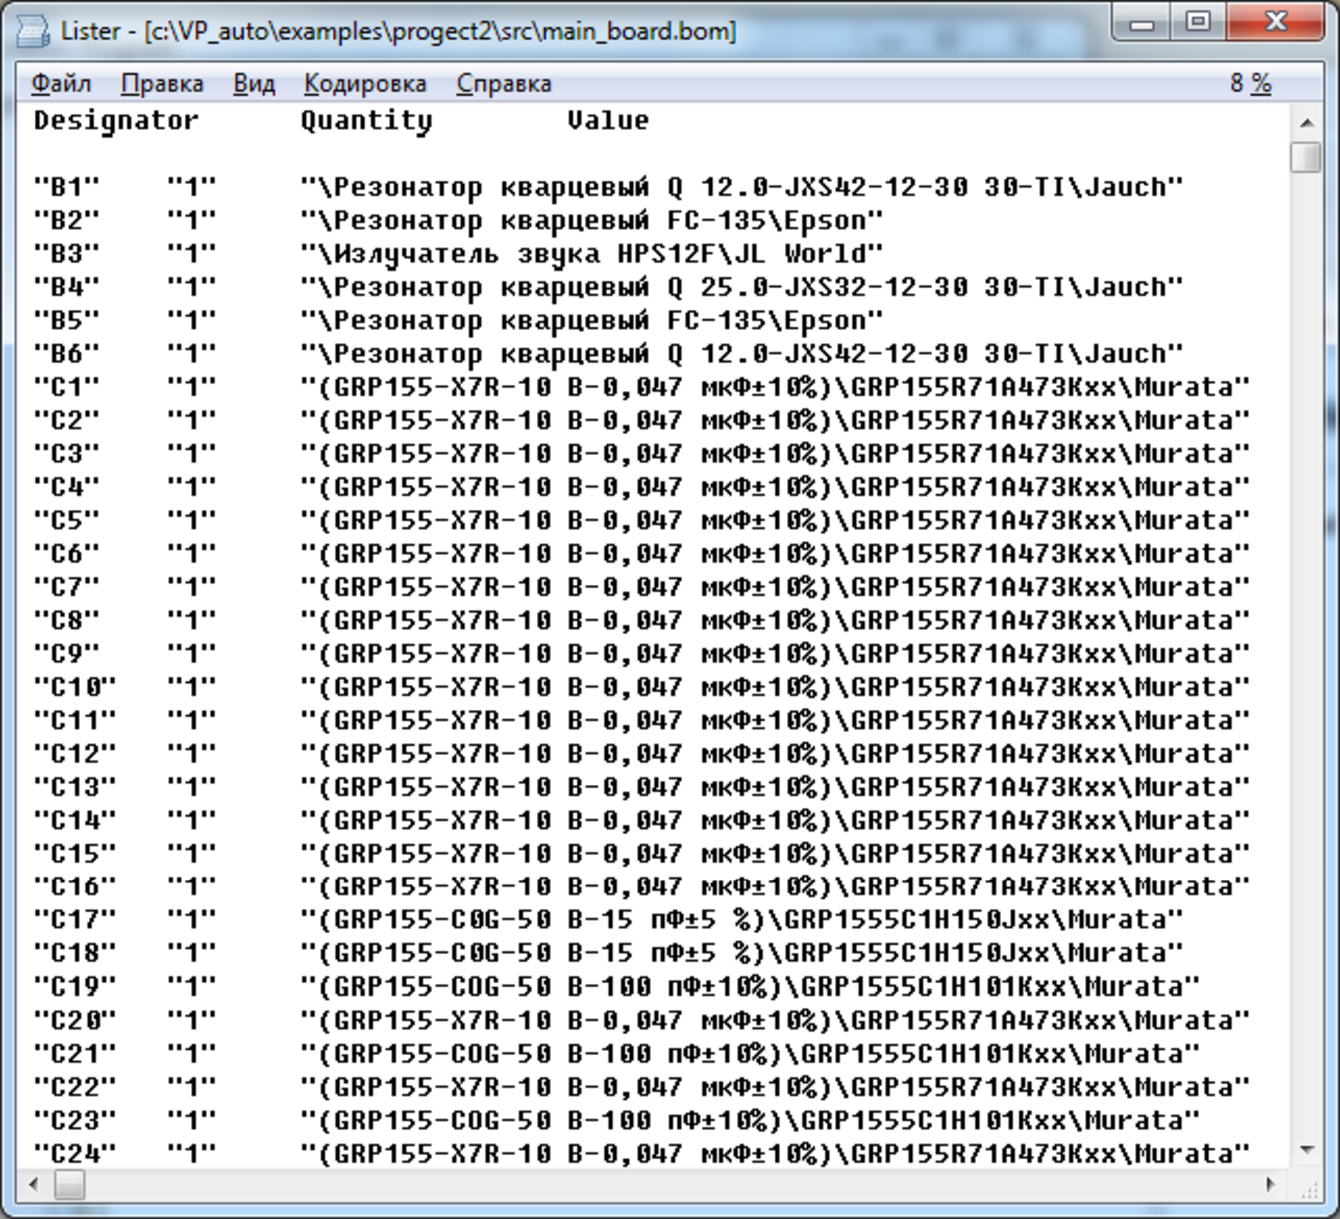
\includegraphics[width=0.8\textwidth]{VP_auto/pictures/ad/pic_ad_low_bom_file}
  \caption{Содержимое ''*.bom''--файла среды ''Altium Designer''} \label{p:pic_ad_low_bom_file}
\end{figure}

Для правильного создания такого файла в среде проектирования ''Altium Designer'' нужно выполнить ниже рекомендуемые действия.

\subsubsection{}Проставить в свойствах каждого элемента в поле \verb|"Value"| текст, который будет фигурировать в ведомости покупных в формате: \\
\fbox{расшифровка\textbackslash код продукта\textbackslash фирма--производитель} \\ \hspace*{20mm} (пример: \fbox{(GRM188-X7R-16В-0,1 мкФ+-20\%)\textbackslash GRM188R71C104Mxx\textbackslash Murata})\\
или \\
\fbox{\textbackslash код продукта\textbackslash фирма--производитель} \\ \hspace*{20mm} (пример: \fbox{\textbackslash 74LVC04 AD\textbackslash Phillips})\\
или \\
\fbox{\textbackslash код продукта\textbackslash технические условия} \\ \hspace*{20mm} (пример: \fbox{\textbackslash Приёмник навигационный\textbackslash АБВГД.123456.074}).

Знак \verb|"\"| является разделителем между полями. Знак \verb|"@"| тоже
зарезервирован. Остальными знаками можно пользоваться. Примерный вид свойств элемента показан на рисунке~\ref{p:pic_ad_component_properties_d}) (для микросхемы и для любого другого элемента, не требующего расшифровки названия) и на рисунке~\ref{p:pic_ad_component_properties_c} (для конденсаторов и для других элементов, требующих расшифровки названия).

\begin{figure}[H]\center
  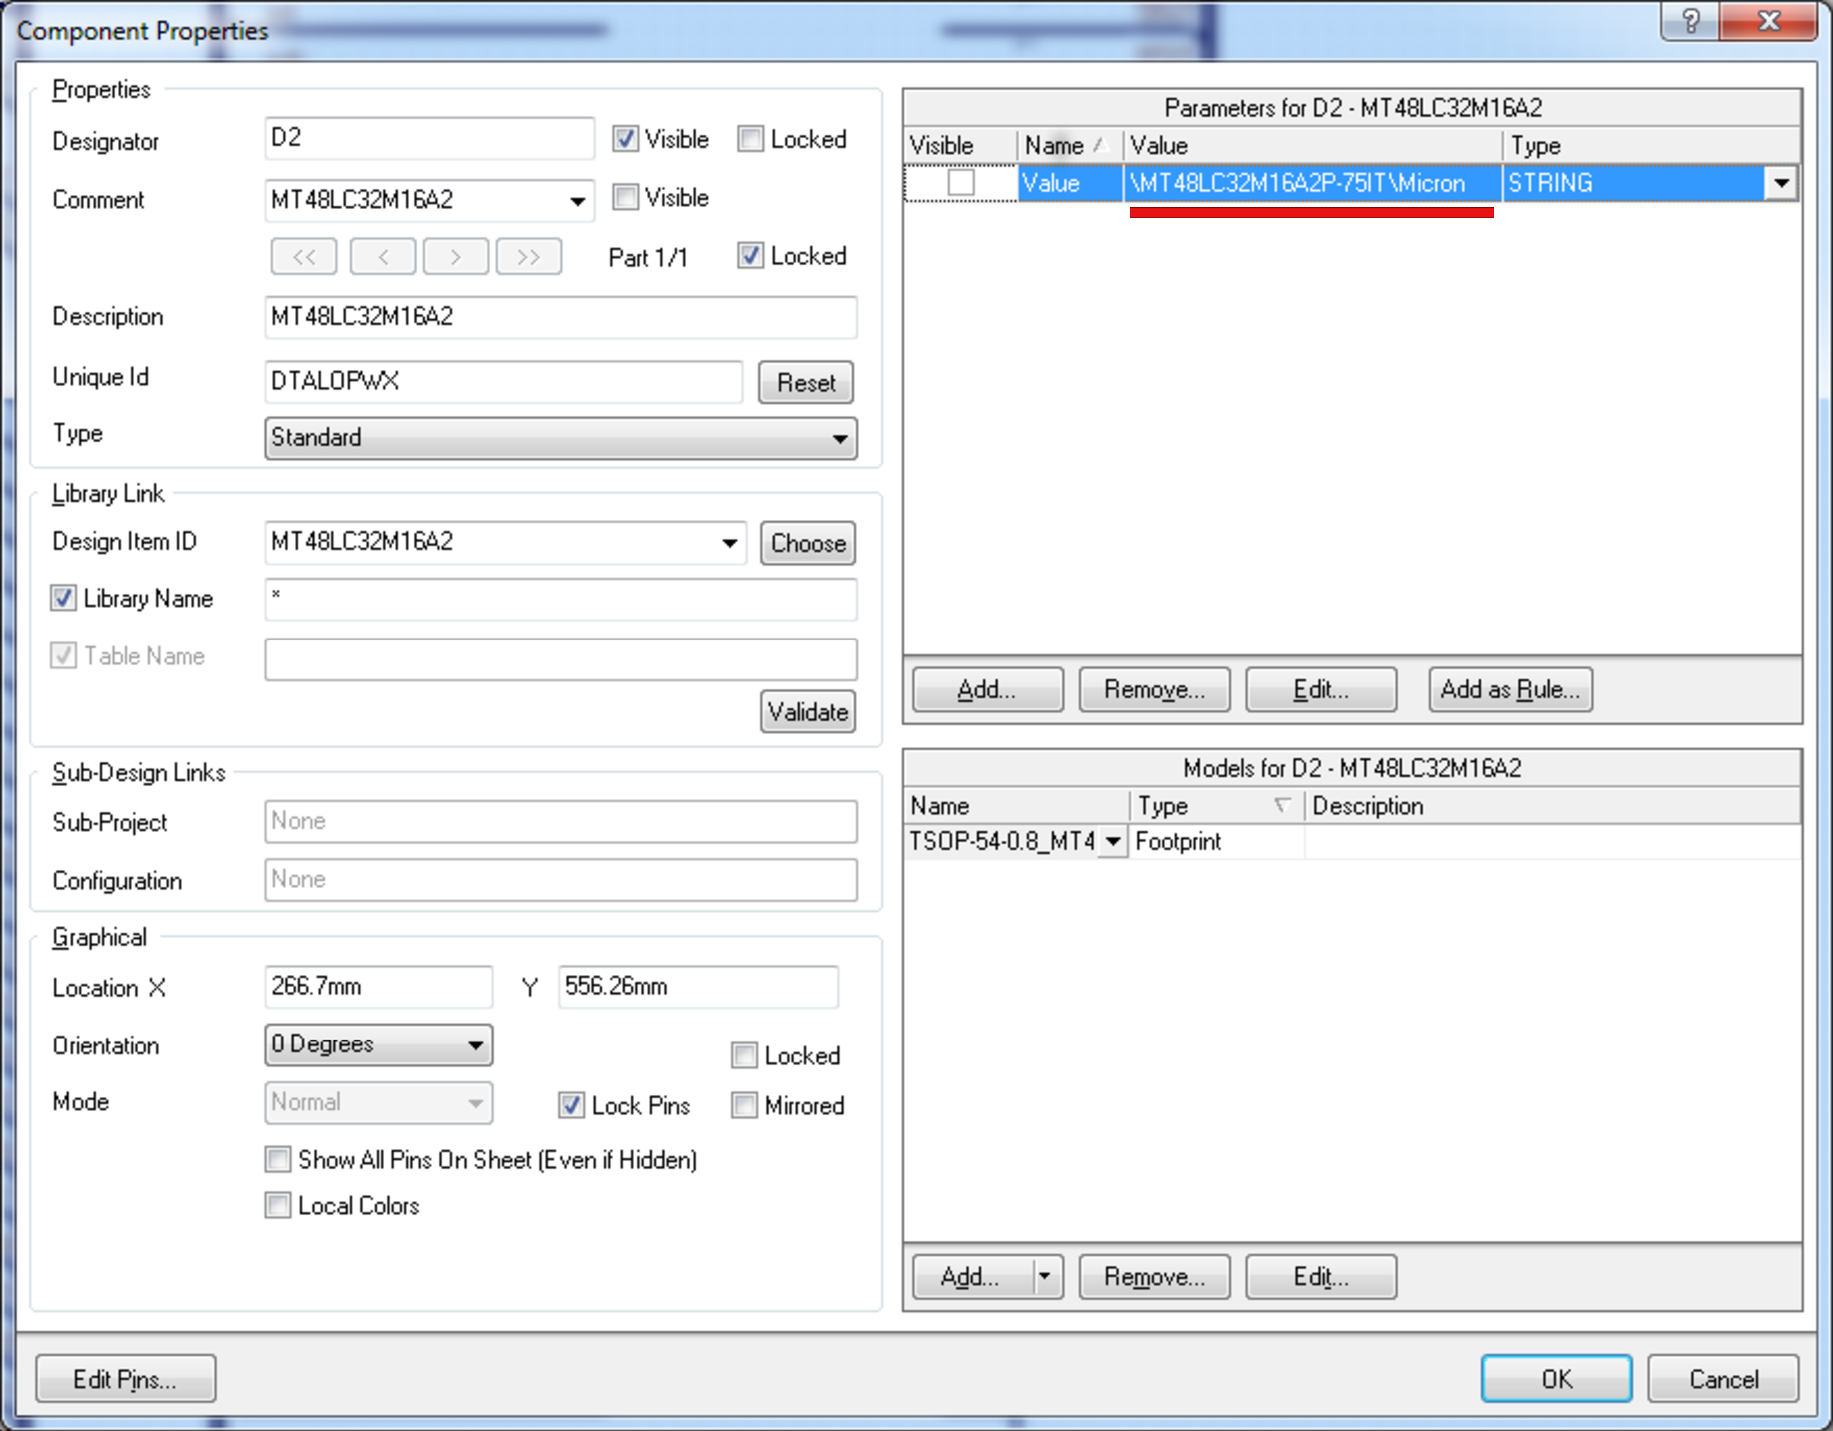
\includegraphics[width=1\textwidth]{VP_auto/pictures/ad/pic_ad_component_properties_d}
  \caption{Окно свойств элемента среды ''Altium Designer''} \label{p:pic_ad_component_properties_d}
\end{figure}

\newpage
\begin{figure}[H]\center
  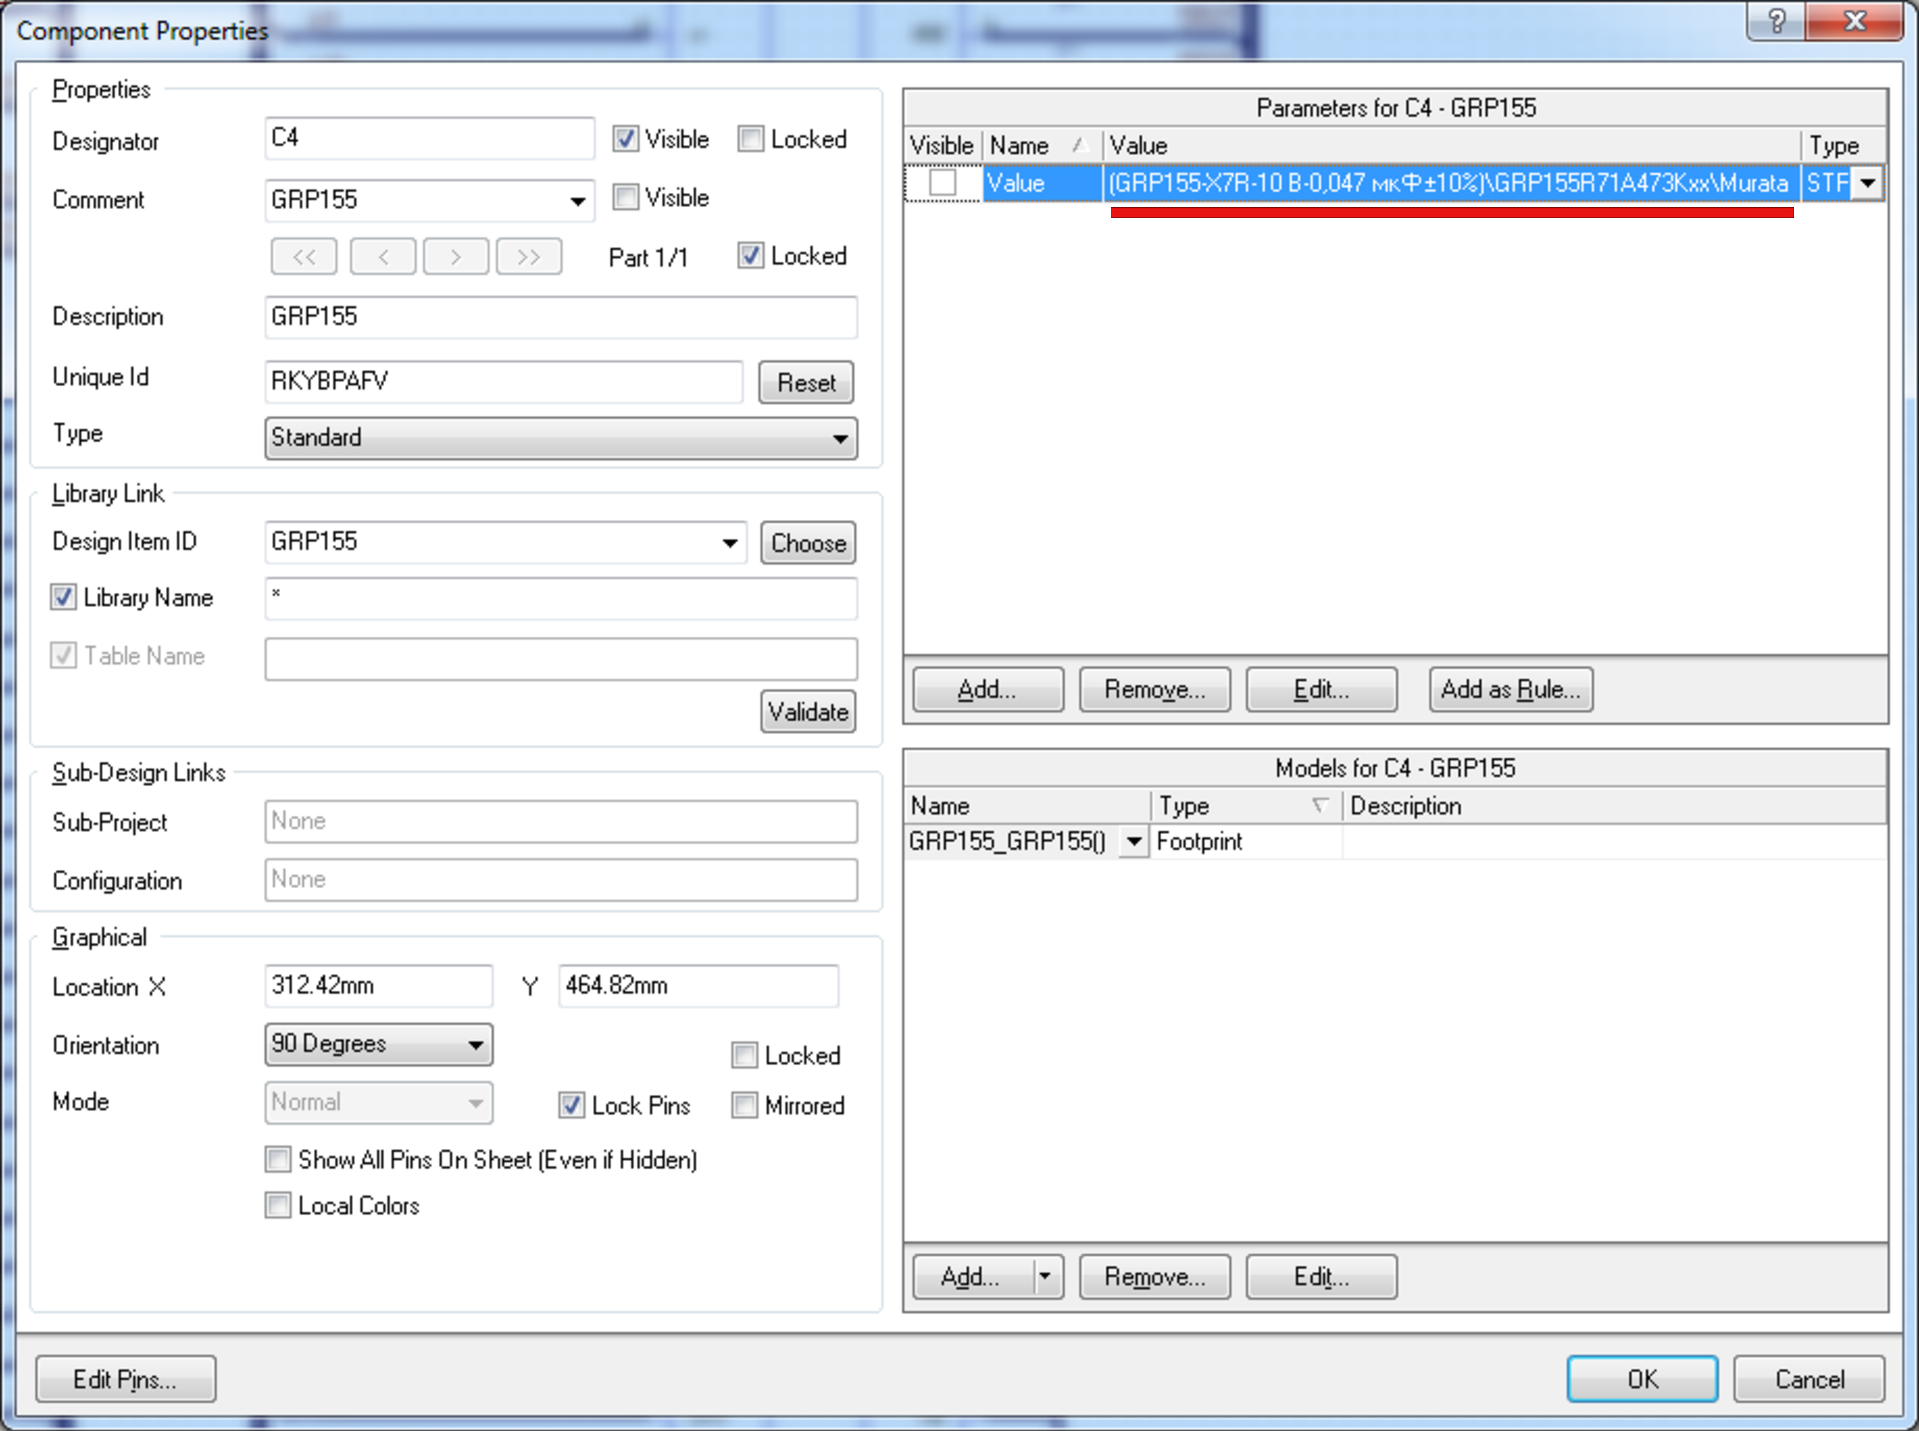
\includegraphics[width=1\textwidth]{VP_auto/pictures/ad/pic_ad_component_properties_c}
  \caption{Окно свойств элемента среды ''Altium Designer''} \label{p:pic_ad_component_properties_c}
\end{figure}

\newpage
\subsubsection{}Настроить параметры файла отчёта. Заходим в \\ \verb|"Reports->Bill of Materials..."|
и устанавливаем настройки согласно рисунку~\ref{p:pic_ad_bom_creater_window}.

\begin{figure}[H]\center
  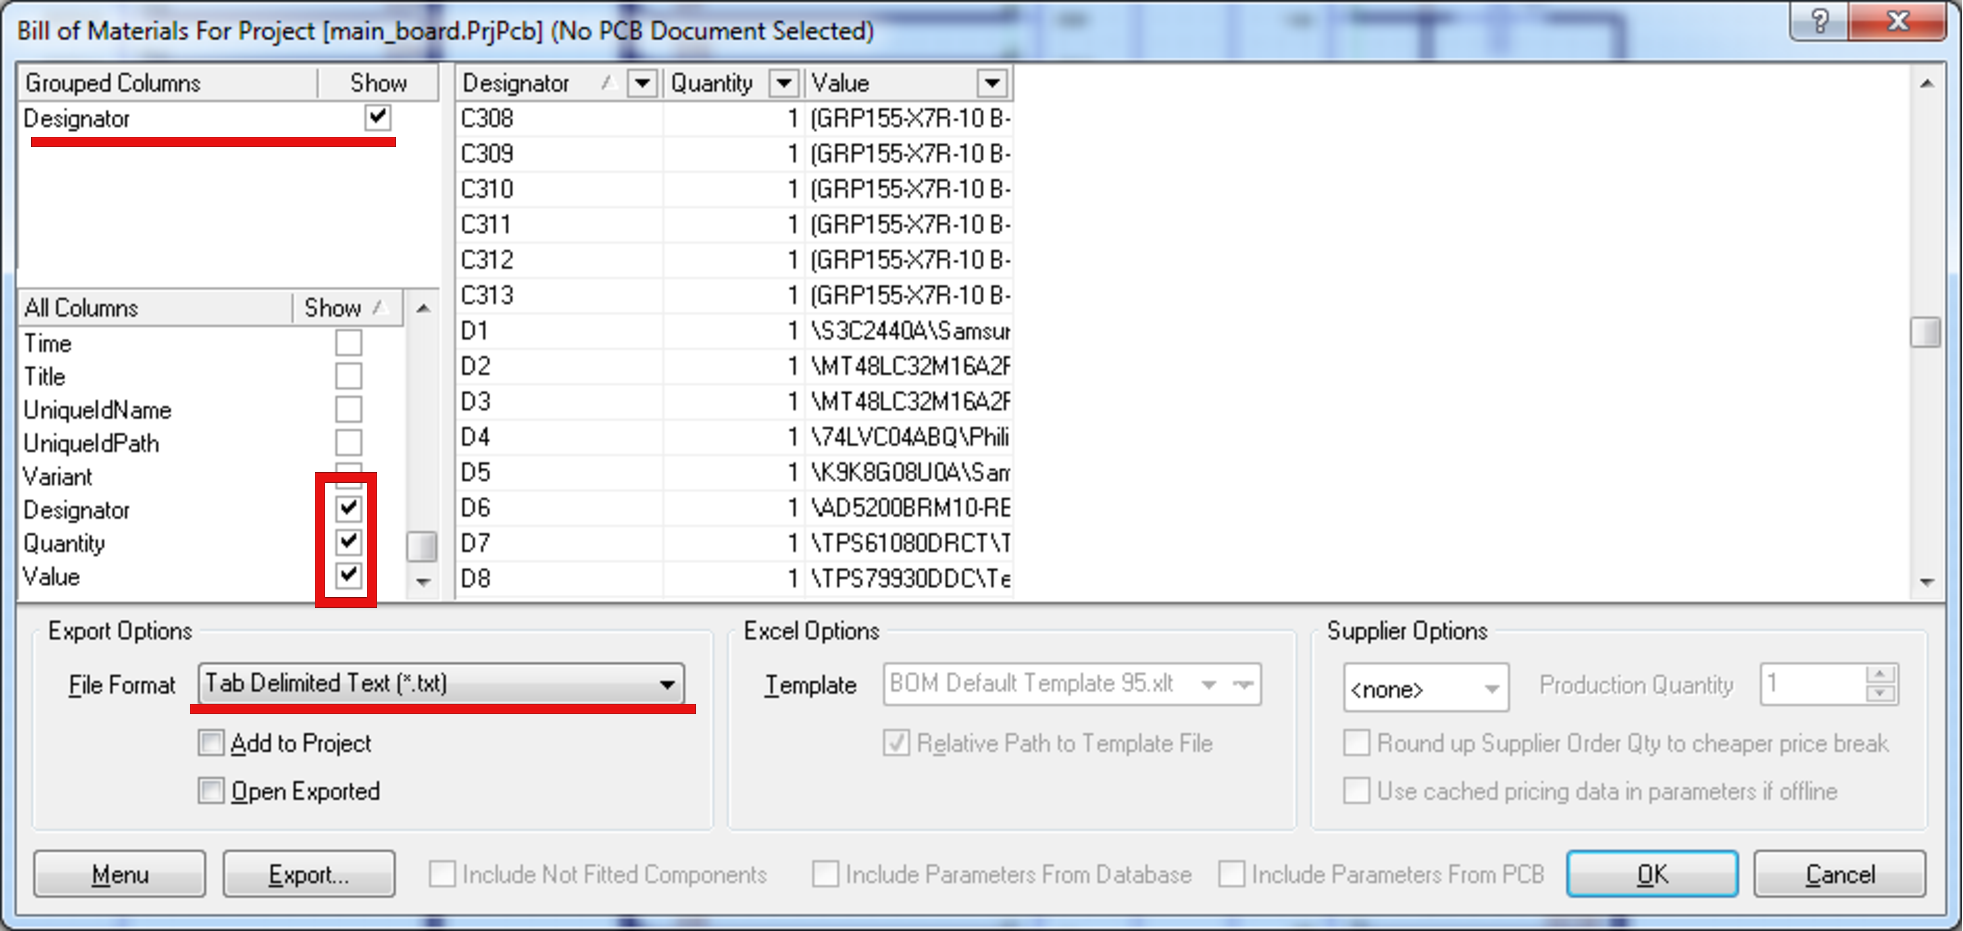
\includegraphics[width=1\textwidth]{VP_auto/pictures/ad/pic_ad_bom_creater_window}
  \caption{Окно настройки файла отчёта среды ''Altium Designer''} \label{p:pic_ad_bom_creater_window}
\end{figure}

\subsubsection{}Проделываем аналогичные операции с остальными файлами.

Отметим, что в среде ''Altium Designer'' есть возможность добавить поля \\''фирма--производитель'', ''расшифровка'' на видное место и,
как следствие, получить более удобочитаемый файл отчёта, но автор не видит в этом сильной необходимости. В дальнейшем возможно введение в программу поддержки нескольких видов файлов отчётов ''Altium Designer''.






%%%%%%%%%%%%%%%%%%%%%%%%%%%%%%%%%%%%%%%%%%%%%%%%%%%%%%%%%%%%%%%%%%%%%%%

\section{Файл соответствий}\label{sec:detimal} \sectionmark{Файл соответствий}

Файл соответствий (\verb|"*.do"|) предназначен для определения соответствий между децимальными номерами блоков и соответствующих им файлов отчётов. Обычно, сначала схемы начинают разрабатываться а затем занимаются децимальные номера, которые трудно запоминаются. Если переименовать схемы согласно децимальным номерам, то в результате приходится каждый раз открывать все подряд схемы в поисках нужной. Использование файла соответствий решает эту проблему.

Примерный вид файла показан на рисунке~\ref{p:pic_vp_auto_do_file}

\begin{figure}[H]\center
  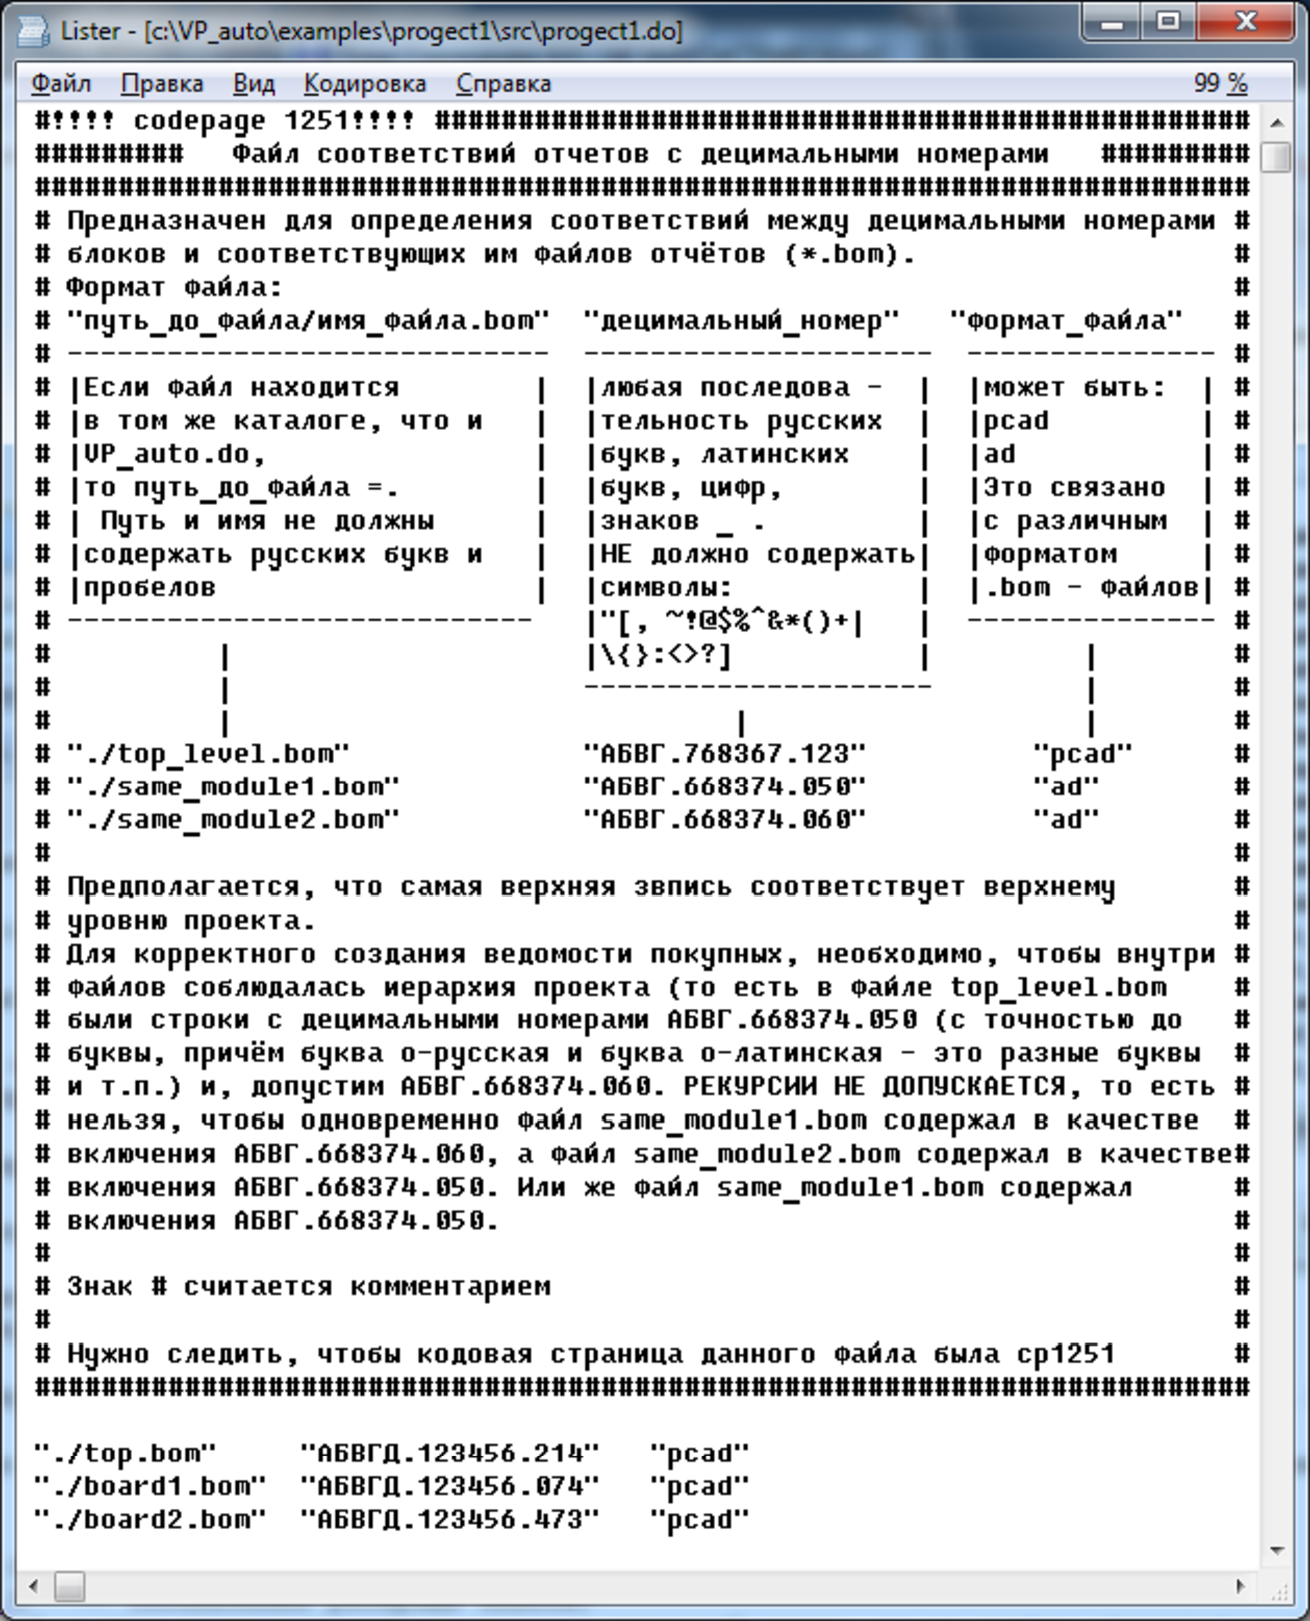
\includegraphics[width=0.8\textwidth]{VP_auto/pictures/pic_vp_auto_do_file}
  \caption{Файл соответствий имён} \label{p:pic_vp_auto_do_file}
\end{figure}

\newpage
Пустые строки и строки, начинающиеся со знака ''\#'' игнорируются. Также игнорируются неполные строки и строки с непотребными символами.

В первой строке этого файла должен быть прописан верхний уровень иерархии, то есть блок, в который в конечном счёте, войдут все остальные блоки. Ведомость покупных создаётся для этого блока. Файл отчёта (\verb|"*.bom"|) верхнего уровня должен содержать децимальные номера входящих в его состав блоков (рисунок~\ref{p:pic_pcad_top_bom_file})

\begin{figure}[H]\center
  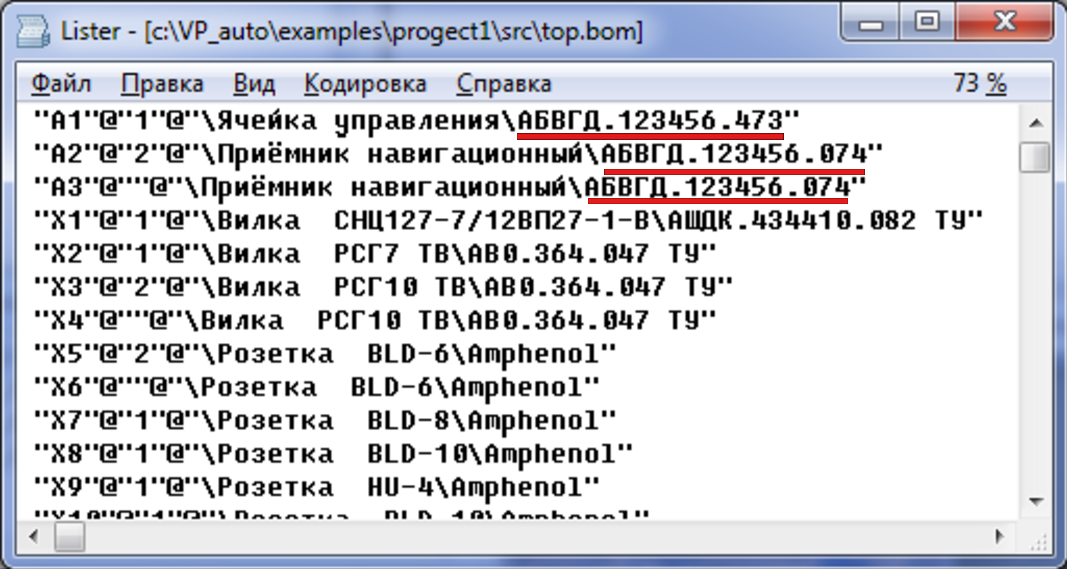
\includegraphics[width=0.8\textwidth]{VP_auto/pictures/pcad/pic_pcad_top_bom_file}
  \caption{Файл отчёта верхнего уровня} \label{p:pic_pcad_top_bom_file}
\end{figure}

Децимальные номера блоков, перечисленные в файлах отчётов (\verb|"*.bom"|), должны в точности совпадать с номерами, приведёнными в (\verb|"*.do"|) -- файле.

Если в файле отчёта прописан не обозначенный в файле соответствий блок, то содержимое этого блока остаётся не раскрытым в ведомости покупных. В ней останется строка с названием, децимальным номером и количеством таких блоков на изделие.



%%%%%%%%%%%%%%%%%%%%%%%%%%%%%%%%%%%%%%%%%%%%%%%%%%%%%%%%%%%%%%%%%%%%%%%%%%%%

\section{Командный файл} \label{sec:comand_file}
\sectionmark{Командный файл}

Программе нужно знать имя обрабатываемого \verb|"*.do"| -- файла. Это имя передаётся
через опции командной строки. Удобно создать командный файл (\verb|"*.bat"|), запускающий программу \verb|"vp_auto.exe"| с именем обрабатываемого файла. Содержимое \verb|"*.bat"| -- файла показано ниже  в листинге.

%\begin{minted}{c}
\inputminted[fontsize=\small, linenos, breaklines, numbersep=2mm, xleftmargin=5mm, frame=single]{bat}{./VP_auto/inc/progect1.bat}
%\end{minted}



%%%%%%%%%%%%%%%%%%%%%%%%%%%%%%%%%%%%%%%%%%%%%%%%%%%%%%%%%%%%%%%%%%%%%%%%%%%%%

\section{Файлы заготовок документов}
\sectionmark{Файлы заготовок документов}

Файлы \verb|"per_auto.sch"|, \verb|"per_canvas_i1.sch"|, \verb|"sp_auto.sch"|, \verb|"vp_auto.sch"|, \verb|"pilot_canvas.sch"|  служат заготовками для создания перечней элементов, спецификаций, ведомостей покупных и др... На рисунке~\ref{p:pic_vp_canvas_file} показан один из этих файлов, открытый стандартным блокнотом.

\begin{figure}[H]\center
  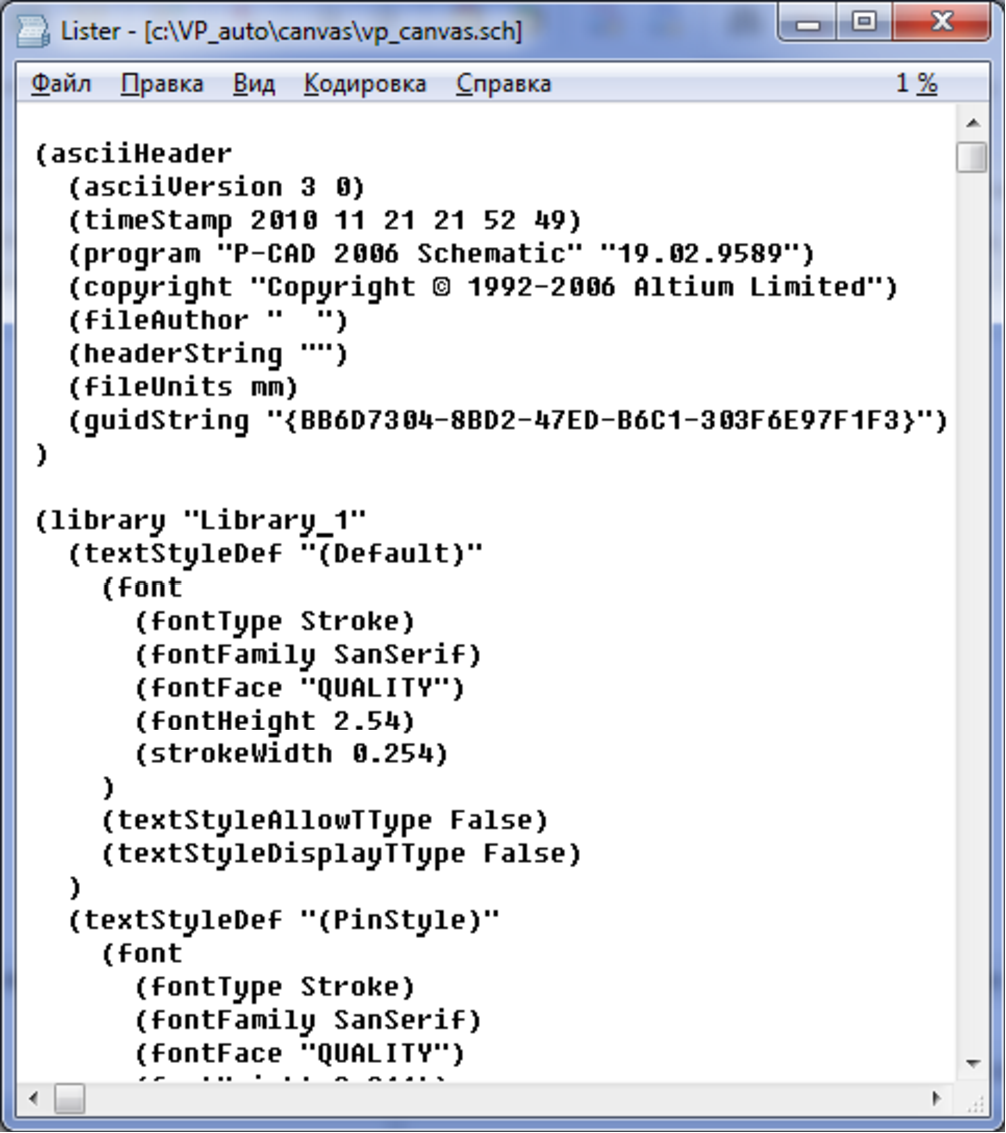
\includegraphics[width=0.8\textwidth]{VP_auto/pictures/pic_vp_canvas_file}
  \caption{Файл -- заготовка, открытый блокнотом} \label{p:pic_vp_canvas_file}
\end{figure}

Программа копирует строки из файлов -- заготовок в созданные проектные файлы и заодно вписывает свою информацию. В результате, выше перечисленные документы создаются в формате ''P-CAD 2006 SP2 Shematic''. Применение данного формата для документов аргументировано следующими соображениями:
\begin{itemize}
  \item вместо традиционно использующейся в данном случае связки ''P-CAD 2006 SP2'' + ''MS World'' для хранения файлов схемы и перечня остаётся только один;
  \item данный формат является по сути векторным многостраничным документом с открытой структурой, поддержкой шрифтов семейства TrueType и идеологией xml (к примеру, открытый векторный формат \verb|"svg"| так и остаётся одностраничным, формат \verb|"dxf"| не поддерживает шрифты TrueType);   
  \item спецификация, сделанная в пакете ''Компас'' хоть и выглядит красиво, но трудно поддаётся редактированию, связанному с перестановкой записей;
  \item значительному упрощению кода программы, из--за отсутствия необходимости расшифровывать бинарные форматы файлов ''Компас'' или ''MS Office'' или использовать OLE -- технологию;
  \item вообще у автора негативное отношение к продукту ''MS World''  из -- за его непредсказуемости особенно заметной на многостраничных документах, насыщенных картинками, таблицами и формулами (сформировавшееся ещё со времён студенчества). Для справки -- данный документ создан с помощью издательской системы LaTeX (TeX~Live~2016).
\end{itemize}

Анализ вариант экспорта файлов в формат LaTeX показал нецелессообразность данного мероприятия. Там получается здоровая многостраничная таблица с элементами в названиях которых будет куча экранирующих символов. В результате чуть что не так -- можно много времени потерять на выяснение причин почему LaTeX отказывается верстать сие (поверьте мне, как автору eskdi)... Это противоречит идеологии минимизации времени на рутину.

Возможно стоит проанализировать xml -- формат LibreOffice.


%%%%%%%%%%%%%%%%%%%%%%%%%%%%%%%%%%%%%%%%%%%%%%%%%%%%%%%%%%%%%%%%%%%%%%%%%%%%%

\section{Файлы ресурсов}
\sectionmark{Файлы ресурсов}

Под файлами ресурсов подразумеваются файлы, которые редактирует пользователь программы с целью минимизировать ошибки, возникающие при вводе названий лементов с клавиатуры.

По умолчанию, файлы ресурсов расположены в папке \verb|"VP_auto/res"|). Путь к папке с ресурсами можно переопределить из командной строки программы.



\subsection{Файл ''./res/firms.txt''}
Файл \verb|"firms.txt"| содержит утверждённые местным нормоконтролем названия фирм и технических условий. Каждое название в новой строчке. Знак '\#' в начале строки -- строка комментариев. Кодировка файла -- UTF-8. Примерный вид файла приведён в листинге ниже.

%\begin{minted}{c}
\inputminted[fontsize=\small, linenos, breaklines, numbersep=2mm, xleftmargin=5mm, frame=single]{bash}{./VP_auto/inc/firms.txt}
%\end{minted}




\subsection{Файл ''./res/names.txt''}
Файл \verb|"names.txt"|. Знак '\#' в начале строки -- строка комментариев. Кодировка файла -- UTF-8. Примерный вид файла приведён в листинге ниже.

%\begin{minted}{c}
\inputminted[fontsize=\footnotesize, linenos, breaklines, numbersep=2mm, xleftmargin=5mm, frame=single]{bash}{./VP_auto/inc/names.txt}
%\end{minted}



\subsection{Файл ''./res/true\_elements.txt''}
Файл \verb|"true_elements.txt"| содержит согласованные на данный момент названия элемента (со знаком '+'), ранее применяемые названия элемента (со знаком '-'). Знак '\#' в начале строки -- строка комментариев. Кодировка файла -- UTF-8. Примерный вид файла приведён в листинге ниже.

%\begin{minted}{c}
\inputminted[fontsize=\small, linenos, breaklines, numbersep=2mm, xleftmargin=5mm, frame=single]{text}{./VP_auto/inc/true_elements.txt}
%\end{minted}






%%%%%%%%%%%%%%%%%%%%%%%%%%%%%%%%%%%%%%%%%%%%%%%%%%%%%%%%%%%%%%%%%%%%%%%%%%%%

\section{Порядок работы с программой}
\sectionmark{Порядок работы с программой}

Для того, чтобы подготовить свой проект необходимо проделать следующие действия:
\begin{enumerate}
  \item создать папки \verb|"my_path/"|, \verb|"my_path/src/"|;
  \item создать файлы отчётов как показано в п.~\ref{sec:reports} для всех схем проекта и переместить их в папку \verb|"my_path/src/"|;
  \item создать файл соответствий согласно своему проекту, п.~\ref{sec:detimal} и поместить его в папку \verb|"my_path/src/"|;
  \item создать командный файл в папке \verb|"my_path/"|, отредактировать командный файл согласно п.~\ref{sec:comand_file} (правильно указать пути к исполняемому файлу \verb|"vp_auto.exe"| файлу взаимосвязей);
  \item запустить командный файл \verb|"*.bat"|;
  \item открыть файл отчёта о проделанных действиях \\ \verb|"my_path/out/VP_auto_utf8.log"| и проанализировать его содержимое. При нахождении программой замечаний (ошибки в названии элементов), устранить на схемах, перегенерировать файлы отчетов. При необходимости, внести изменения в файлы ресурсов;
  \item запустить командный файл \verb|"*.bat"| вновь;
  \item открыть по очереди созданные \verb|"my_path/out/*.sch"| -- файлы, проанализировать и окончательно отредактировать их;
  \item перенести отредактированные \verb|"my_path/out/*.sch"|  -- файлы в другую папку.
\end{enumerate}

Примеры готовых проектов содержатся в каталоге \verb|"VP_auto/examples/"| (нужно только запустить командные файлы).

%%%%%%%%%%%%%%%%%%%%%%%%%%%%%%%%%%%%%%%%%%%%%%%%%%%%%%%%%%%%%%%%%%%%

\section{Принцип действия программы}
\sectionmark{Принцип действия программы}

Программ \verb|"vp_auto.exe"| считывает содержимое файлов, прописанных в \\ \verb|"*.do"|, присваивает каждой записи из файлов соответствующий децимальный номер блока куда входит этот элемент, избавляется от мусора, сортирует по категориям, по алфавиту, объединяет некоторые строчки. Затем объединяет полученную информацию и информацию из \verb|"*_canvas.sch"| -- файлов в соответствующие файлы \verb|"my_path/out/*.sch"|, \verb|"my_path/out/*ПЗ3.sch"| и \verb|"my_path/out/*ВП.sch"|. Затем производит анализ схожести названий элементов между собой и с эталонными списками.

%%%%%%%%%%%%%%%%%%%%%%%%%%%%%%%%%%%%%%%%%%%%%%%%%%%%%%%%%%%%%%%%%%%%

\section{Список изменений}
\sectionmark{Список изменений}

''V~3.0'':
\begin{enumerate}
\item полностью переработан алгоритм создания спецификаций, перечней элементов, ведомости покупных;
\item добавлен алгоритм создания перечня элементов для включения в приложения инструкций в виде картинок (скажем, инструкций по проверке, сделанных в eskdi);
\item добавлен алгоритм формирования бирок с названием и количеством элементов (для облегчения труда комплектовщиков в сборочном цехе);
\item полностью переделан интерфейс командной строки (код сгенерирован с помощью GNU~Gengetopt);
\item сделана более гибкая раота с каталогами;
\item корректная работа с русскими буквами в путях к файлам;
\item при создании документации используются классы, вычисляющие длину текста, написанную определённым шрифтом (GOST~type~B);
\item добпален алгоритм распознавания типа элемента из названия элемента (основан на значении Ref и содержимом ресурсного файла \verb|"VP_auto/res/names.txt"|);
\item добавлен алгоритм сравнения названия фирмы элемента с эталонным списком фирм (файл \verb|"VP_auto/res/firms.txt"|);
\item добавлен алгоритм сравнения кода элемента с эталонным списком элементов (файл \verb|"VP_auto/res/true_elements.txt"|);
\item улучшен алгоритм поиска в проекте одинаковых элементов, записанных не одинаковым образом;
\item добавлен модуль, экспортирующий структуру проекта (какая сборка в какую сборку входит) в \verb|"*.dot"| -- файл, который можно преобразовать в \verb|"*.pdf"| или \verb|"*.jpg"| с помощью пакета Graphviz или открыть векторным редактором Inkscape;
\item сильно переработан исходный код в сторону оптимизации и читаемости;
\item программа переведена на QT5.6.
\end{enumerate}

''V~2.5'':
\begin{enumerate}
  \item полностью переработан алгоритм создания спецификаций, устранён глюк с пропуском некоторых позиций в спецификации;
  \item содержимое лог--файла теперь на русском языке, доступно для понимания и анализа;
  \item добавлена обработка исключительных ситуаций при разборе содержимого входных файлов \verb|"*.do"| и \verb|"*.bom"| (все сообщения отправляются в файл отчёта);
  \item введена возможность работы с ''Altium Designer'';
  \item в \verb|"*.do"| -- файл добавлен новый столбец (формат \verb|"*.bom"| -- файла) и справочная информация;
  \item программа тестировалась на проекте с количеством покупных изделий более 1000 (более 100 наименований);
  \item проект переведён на QT5;
\end{enumerate}

''V~2.0a'' -- базовая версия.


%%%%%%%%%%%%%%%%%%%%%%%%%%%%%%%%%%%%%%%%%%%%%%%%%%%%%%%%%%%%%%%%%%

\section{Особенности работы программы}
\sectionmark{Особенности работы программы}

\begin{enumerate}
  \item Программа тестировалась со средой ''P-CAD 2006 SP2''.  Данная версия продукта корректно производит сохранение и разборку собственных ASCII--файлов (нет проблем со знаком ''я'', как в предыдущих версиях продукта);
  
  \item В программе \textbf{нет обработки рекурсий}. Программа будет вылетать при попытке включить блок сам в себя или если два блока включают друг друга;
    
  \item Для ''P-CAD 2006'' элементы со значением \\
\verb|(GRM188-X7R-16В-0,1 мкФ+-20%)\GRM188R71C104Mxx\Murata|\\
и\\
\verb|(GRM188-X7R-16В-0,1 мкФ+-20%)\GRM188R71C104Mxx \Murata|\\
(добавлен незаметный пробел) являются разными. Соответственно это отразится во всех документах. Для обнаружения опечаток подобного рода в программе заложено несколько алгоритм распознавания схожих записей с занесением результатов в файл отчёта;

  \item Элементы не отображаются в документации, если позиционные обозначения ''RefDes'' их начинаются со значений:
    \itemb ''KT'' -- контрольная точка для местного нормоконтроля;
    \itemb ''REF'', ''REF\_P'', ''REF\_G'' -- обозначения реперных знаков;
    \itemb ''UNUZED'' -- элемент, который должен присутствовать на схеме и печатной плате, но не должен присутствовать в документации (пустое посадочное место под элемент на печатной плате);
    \itemb ''\, '' -- паяные контакты с численными обозначениями (по правилам местного нормоконтроля);
  \item Элементы не отображаются в перечне элементов, но отображаются в спецификации и ведомости покупных, если позиционные обозначения ''RefDes'' их начинаются со значения ''COMPO'' (держатель вставки плавкой, колпачок на соединитель, радиатор, крепление радиатора и др..).
\end{enumerate}



%%%%%%%%%%%%%%%%%%%%%%%%%%%%%%%%%%%%%%%%%%%%%%%%%%%%%%%%%%%%%%%%%%%%%%

\section{Лицензия}
\sectionmark{Лицензия}

Программа распространяется ''как есть'' разработчик не требует за использование плату, и ответственности не несёт в случае утери или повреждения данных. Используйте программу на свой страх и риск. За подробностями обращайтесь по адресу \verb|"https://www.gnu.org/licenses/gpl-3.0.html"|.



%%%%%%%%%%%%%%%%%%%%%%%%%%%%%%%%%%%%%%%%%%%%%%%%%%%%%%%%%%%%%%%%%%%%%%%

\section{Дополнение}
\sectionmark{Дополнение}

Программа собрана в среде \verb|"Qt Creator (open source)"|. Это интегрированная среда для разработки прикладных программ с графическим
интерфейсом для платформ IBM PC и не только... Окошко \verb|"О программе"| показано на рисунке~\ref{p:pic_about_qt}.

\begin{figure}[H]\center
  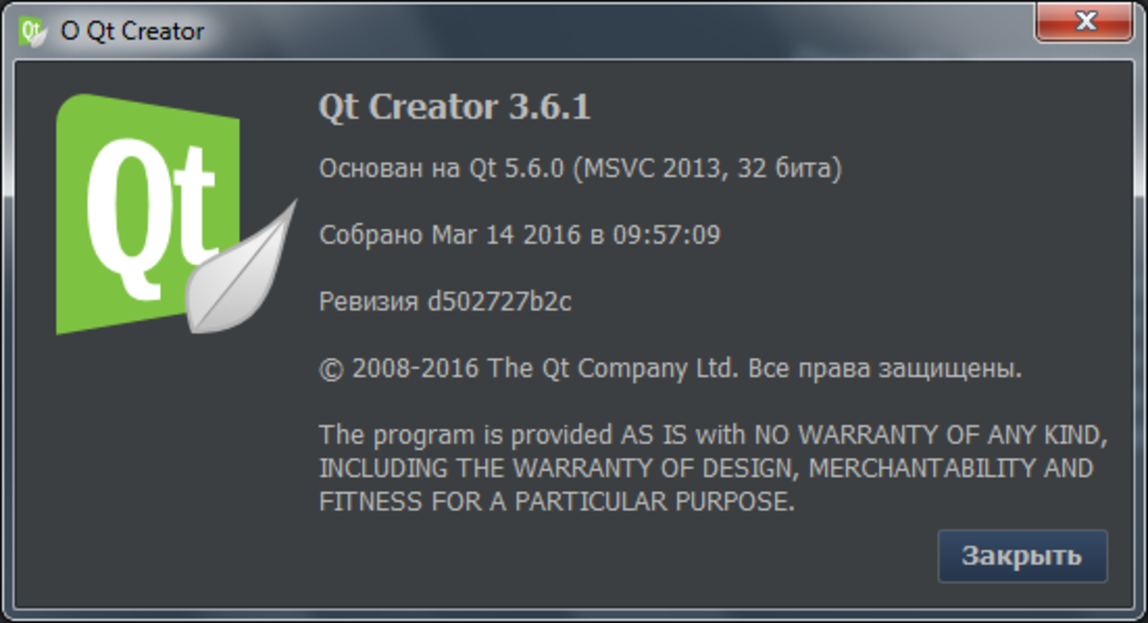
\includegraphics[width=0.8\textwidth]{VP_auto/pictures/pic_about_qt}
  \caption{Среда QT Creator} \label{p:pic_about_qt}
\end{figure}

%%%%%%%%%%%%%%%%%%%%%%%%%%%%%%%%%%%%%%%%%%%%%%%%%%%%%%%%%%%%%%%%%%%%%%%

\section{Пожелания}
\sectionmark{Пожелания}

Надеюсь, эта программа поможет Вам:
\begin{itemize}
  \item избавиться от рутины;
  \item минимизировать число ошибок при сборке печатных плат на производстве;
  \item освободить время для творчества;
  \item получить экономический эффект.
\end{itemize}


С уважением,    Юра Степаненко  \verb"stepanenkoyra@gmail.com".

\end{document}
